% !TeX root = ../Thesis.tex

%************************************************
\chapter{Background}\label{ch:background}
%************************************************
\glsresetall % Resets all acronyms to not used

In this chapter, we want to take a dive into the historical backgrounds of both steganography and \glspl{LLM}. We will investigate how they relate to adjacent fields and how they contribute to problems we are facing today. This deepens our understanding for the underlying motivation of this thesis and explains the requirements for our implementation.

\section{Steganography}
\label{sec:steganography}
This section will first explain the origins of steganography, show positive and negative use cases, and justify its relevance for the general public by involving some politics. Then the foundation for a common understanding is laid by giving all relevant definitions surrounding steganography and by distinguishing it from other fields.

\subsection{From physical to digital steganography}
\label{sec:fromPhysicalToDigitalSteganography}
The term "steganography" originates from ancient Greece and can be translated to "hidden writing"~\cite{kolataVeiledMessagesTerror2001,dembartEndUserHide2001} or "covered writing"~\cite{salleeModelBasedSteganography2004,petitcolasInformationHidingSurvey1999,bennettLinguisticSteganographySurvey2004}. Fundamentally, steganography is an umbrella term for information hiding techniques~\cite{bennettLinguisticSteganographySurvey2004}. When it was first coined by German polymath and early cryptographer Johannes Trithemius in his work "Steganographia" around 1500 A.D., steganography had already been in practice for at least a thousand years~\cite{bennettLinguisticSteganographySurvey2004}. Old Greek historian Herodotus documented it as early as 440 B.C.: Histiaeus, tyrant ruler of Miletus, was being held captive and wanted to send a message to his ally, Aristagoras. Since he had to bypass the guards of his enemies, the message had to be secret. He decided to shave the head of his most trusted slave, tattoo the message onto his scalp and wait for the hair to grow back before sending him on his way. With the message obscured, the slave would arrive at his destination, only for his hair to be shaved off again to read the secret message back~\cite{bennettLinguisticSteganographySurvey2004,petitcolasInformationHidingSurvey1999,dembartEndUserHide2001}.

This technique was still used by German spies until the early twentieth century~\cite{petitcolasInformationHidingSurvey1999}. Similarly, Nazi Germany used microdots in World War II: They shrunk pages of text down to the size of the dots in letters i or j, periods or commas, and sent in printed letters. Invisible to the naked eye, an impressive information density was achieved this way~\cite{dembartEndUserHide2001,petitcolasInformationHidingSurvey1999}.

Today not physical objects, but digital data is used to hide information~\cite{bennettLinguisticSteganographySurvey2004}. Use of digital steganography gained public attention as early as the year 2001, with Osama bin Laden encoding orders to members of his terrorist group, Al-Qaeda, as secret messages in digital files~\cite{dembartEndUserHide2001,schneierTerroristsSteganography2001}. This included maps with targets of terrorist attacks and instructions on how to perform them~\cite{schneierTerroristsSteganography2001}. As information was hidden in the cover media, the terrorists were able to use the public internet as communication channel, without needing to meet or even know each other~\cite{schneierTerroristsSteganography2001}. Steganographic communication therefore can be highly anonymous, asynchronous and resilient, once a communication protocol is established~\cite{schneierTerroristsSteganography2001}. In 2001, an estimated 0.6\% of images posted on auction and, most notably in this context, pornography sites on the internet contained steganographic messages attributed to the terrorist group~\cite{kolataVeiledMessagesTerror2001}. Al-Qaeda was actively using these exact methods in Germany at least up until 2012~\cite{robertsonDocumentsRevealQaedas2012}. This suggests that any internet user active during this time period is likely to have come across their communication without being aware of it, maybe even having distributed some of it further by storing and sharing it.

\subsection{The problems of today}
\label{sec:theProblemsOfToday}
Contrary to what one might think after reading the previous paragraphs, steganography is not only interesting to tyrants, Nazis, terrorists and academics. In this section, we will show how it can be beneficial to the general public.

With the rise of the internet, we feel constantly connected to everyone around us. The commercialization of the internet has created complex power dynamics between governments, corporations and the public. This is a paradigm entirely new in human history, where rules and norms as we know them are largely untested.

Digitalization has unlocked vast potentials for businesses to create new markets, access new regions and innovate their products and processes. Businesses store a lot of sensitive data about users to understand their behaviour, problems and desires, in the name of improving their products~\cite{duportailAskedTinderMy2017,titcombMillionsPeoplesDNA2025}. However, this is not without downsides. It arouses interest by governments~\cite{greenwaldNSAPrismProgram2013}, who could utilize such data about their citizens to maintain political power. While it can be used to tackle challenges like the terrorists mentioned earlier, it can also be abused.

In the strive for power, surveillance is a proven tool. We cannot assume ourselves or our allies to be exceptions to this~\cite{macaskillGCHQTapsFibreoptic2013}. In recent years, many democracies have gone through debates about privacy as a human right versus surveillance in the name of security. Most prominently, this was ignited by Edward Snowden's revelations about the global mass surveillance programs of the \gls{NSA}~\cite{greenwaldEdwardSnowdenWhistleblower2013}: Prism~\cite{greenwaldNSAPrismProgram2013}, XKeyscore~\cite{greenwaldXKeyscoreNSATool2013} and Boundless Informant~\cite{greenwaldBoundlessInformantNSAs2013}. More recent examples include the proposed "chat control" measures in the European Union~\cite{danielChatControlEnd2024} and the ban of Apple's Advanced Data Protection in the United Kingdom~\cite{kleinmanUKGovernmentDemands2025,kleinmanApplePullsData2025}. The impact of these affairs is powerful enough to disrupt diplomatic relations between countries and their allies, shifting global power dynamics due to violations of trust~\cite{traynorMerkelComparedNSA2013}.

By governments forming public-private partnerships with software companies in the security sector, surveillance is being commercialized~\cite{bbcPegasusSpywareSold2021,kasterPrivatizedEspionageNSO2023}. Even with legal restrictions on who to sell a spyware product to, it can get into the "wrong" hands. As software is not a physical good, once it's out there, it can't be taken back.

Traditional warfare has expanded into a new dimension, the cyberspace~\cite{serpanosCyberwarfareUkraine2022}. The ability to intercept an enemy's communication in real time can decide the outcome of wars, and therefore about life or death, democracy or dictatorship. For example, this practice is part of the Russian invasion of Ukraine~\cite{sufiSocialMediaAnalytics2023}. Steganography can help conquer this problem by hiding sensitive information in unsuspicious cover media, rendering any messages an attacker could gain access to useless. Similarly it can also help avoid mistakes, thereby improving not just security, but also safety of a communication system. A recent example for this is United States officials accidentally leaking information to a journalist on Signal~\cite{goldbergTrumpAdministrationAccidentally2025,goldbergHereAreAttack2025}.

All of the above considerations culminate in one lesson: We have to be aware of our personal data, that it can be exploited against us, and that we have to protect us against this. To leverage steganography for the public good, we have to understand it. The next section will deliver the relevant definitions surrounding steganography that enable us to do this.

\subsection{Formalizing steganography}
\label{sec:formalizingSteganography}
Steganography is often described as the art and science of hiding information~\cite{bennettLinguisticSteganographySurvey2004,wuGenerativeTextSteganography2024}. As we have seen in \cref{sec:fromPhysicalToDigitalSteganography}, steganography can come in many forms, limited only by our creativity. In this thesis, we want to focus on performing digital steganography, i.e. on hiding data in other data. More specifically, we will focus on text-based or linguistic steganography, i.e. on working with natural language text~\cite{zieglerNeuralLinguisticSteganography2019}.

As we have seen in \cref{sec:theProblemsOfToday}, there are many reasons why one would want to be able to communicate privately. All of the scenarios considered can be traced back to a common denominator: We have two parties, Alice and Bob. They act as sender and receiver, wanting to communicate with each other~\cite{wuGenerativeTextSteganography2024}. While sender and receiver can generally be individuals or systems~\cite{bennettLinguisticSteganographySurvey2004}, we will focus on individuals. To communicate, they send messages to each other. A message is the data or information transmitted between sender and receiver. Furthermore there is an attacker, Eve, who wants to compromise this communication~\cite{al-aniOverviewMainFundamentals2010,wuGenerativeTextSteganography2024}.

In text-based steganography, we say that we encode a secret message into a cover text, thereby hiding it (see \cref{sec:lowLevelManipulatingTokenGeneration} and \cref{ch:implementation} for details). The secret message is something sensitive, i.e. what Alice and Bob actually want to communicate. The cover text is something unsuspicious~\cite{al-aniOverviewMainFundamentals2010}. The cover text is the message being exchanged between Alice and Bob. Alice encodes the secret message into the cover text before sending it to Bob, Bob decodes it back from the cover text after receiving it~\cite{al-aniOverviewMainFundamentals2010}.

To work with this, we need to define objectives and threat models for our communication system. There are various objectives commonly defined in information security. Confidentiality, integrity and availability (collectively known as the "CIA triad") are prominent examples~\cite{aliIoTSecurityReview2019,qadirReviewPaperCryptography2019,chowdhuryChatGPTThreatCIA2023}. But for our use case, we want to focus on the objective of privacy. Privacy can be defined as to ensure that data or information can only be accessed by authorized parties (note that confidentiality can be defined similarly)~\cite{chowdhuryChatGPTThreatCIA2023}. The relevant information is what is hidden in the messages that are being exchanged.

Similarly, there are various aspects one can define about a threat model. Again, we want to focus on what makes our use case unique. We have a key assumption: The attacker can read all messages sent between Alice and Bob. This includes past, present and future messages. Compared to other common threat models (e.g. Dolev-Yao~\cite{dolevSecurityPublicKey1983}), this is a relatively powerful attacker. Therefore, we have a key restriction: The attacker does not know how the steganography works or that it is being used in the first place~\cite{al-aniOverviewMainFundamentals2010}.

This restriction however violates Kerckhoffs' principle: Kerckhoffs demands that a \textit{cryptographic} system should remain secure even if an attacker knows everything about the system, except the secret key~\cite{andersonLimitsSteganography1998,smithEffectiveSecurityObscurity2022} - or as Claude Shannon phrased it: "assume that the enemy knows the system"~\cite{shannonCommunicationTheorySecrecy1949}. The opposite is also called "security through obscurity"~\cite{smithEffectiveSecurityObscurity2022}. In steganography, we don't necessarily deal with secret keys. But as stated in the restriction above, the security of our \textit{steganographic} system partially relies on the attacker's unawareness of the steganography being used~\cite{al-aniOverviewMainFundamentals2010}.

Violating Kerckhoffs' principle is not an issue by itself, if steganography is used correctly: It is not supposed to be used in place of other security mechanisms like authentication, access control and encryption, but in addition to them~\cite{al-aniOverviewMainFundamentals2010}. This is because if we assume the powerful attacker modelled above, steganography is the last layer of security that is left to protect our privacy. Without steganography, there would be no layer left and the communication system would be compromised.

But steganography can also secure a communication channel that doesn't allow any other security mechanisms. This can be demonstrated especially well with text-based steganography, as it has a distinct advantage: It is independent from any one communication medium~\cite{zieglerNeuralLinguisticSteganography2019}. A cover text can be sent digitally as a chat message or in an e-mail, but it can also be spoken during a phone call, hand-written in a letter or printed out in a newspaper. This would be not possible with other types of steganography, e.g. image-based steganography, as those encode information by manipulating redundant binary data~\cite{bennettLinguisticSteganographySurvey2004}. Therefore, text-based steganography can add a layer of security to any communication channel, while other types of steganography can only do this for digital communication channels. In~\cref{sec:fromPhysicalToDigitalSteganography}, we have seen an example for the former with the old Greeks and the Nazis, and an example for the latter with Al-Qaeda.

To introduce our last relevant term, we have to weaken the key restriction of our threat model slightly. If the attacker knows or supposes that steganography is being used, but still doesn't know how it works, they can use steganalysis to try to retrieve the secret message~\cite{bennettLinguisticSteganographySurvey2004}. In general, steganalysis approaches are as diverse as steganography approaches~\cite{bennettLinguisticSteganographySurvey2004}. In text-based steganography, steganalysis is focussed on finding irregularities in the cover texts. This is hard as natural language is irregular, so minor deviations from it are easy to hide in cover texts. While major deviations might be easy to spot in a human steganalysis, the cover texts we can generate today are not prone to such~\cite{wuGenerativeTextSteganography2024}. Therefore we will have to consult machine steganalysis, investigating statistical properties of larger amounts of cover texts than what would be feasible to read and judge manually~\cite{yangSeSyLinguisticSteganalysis2022,wuGenerativeTextSteganography2024}.

\subsection{Relation to other fields}
\label{sec:relationToOtherFields}
In this section, we want to deepen our understanding of what makes steganography unique. First we compare it to the field of cryptography, as both share similar goals. Then we compare it to the field of watermarking, as both share similar mechanisms.

\subsubsection{Cryptography}
\label{sec:cryptography}
While both cryptography and steganography aim to increase security by protecting data from being accessed by an attacker, they do so in fundamentally different ways~\cite{al-aniOverviewMainFundamentals2010,qadirReviewPaperCryptography2019}. Cryptography protects data by encrypting it with a secret key~\cite{qadirReviewPaperCryptography2019}. If Kerckhoffs' principle is followed, this renders the encrypted data useless without knowledge of the secret key~\cite{andersonLimitsSteganography1998,smithEffectiveSecurityObscurity2022}. To an attacker, the encrypted data will look like random noise with no perceivable signal that would contain information~\cite{qadirReviewPaperCryptography2019}. The attacker is only able to make sense of the encrypted data if he obtains the secret key to decrypt it~\cite{malikHighCapacityText2017,qadirReviewPaperCryptography2019}. But when an attacker encompasses encrypted data, it suggests to him that there is secret communication happening~\cite{malikHighCapacityText2017}. This may incentivize the attacker to try and gain access to what is being communicated - if there is something to hide, it might be valuable after all~\cite{malikHighCapacityText2017}. Cryptography is not able to hide data. It answers this problem solely in the spirit of Kerckhoffs, by demanding that we do not have to hide it in the first place~\cite{malikHighCapacityText2017,qadirReviewPaperCryptography2019}.

Steganography uses a different approach. As a mechanism to hide data, it tries to deflect the attacker's attention elsewhere~\cite{al-aniOverviewMainFundamentals2010}. If steganography is performed \textit{after} encryption, the attacker may be able to read the cover text, but they should think that there is no secret communication happening - if there is nothing to hide, there can't be anything of value after all. This would be the success scenario for steganography. Effectively, steganography tries to secure communication by creating covert channels~\cite{gaureL^2M^2C^22024}.

This doesn't mean we have to do without encryption, as we can encrypt the secret message \textit{before} encoding it in the cover text. This fits steganography into the common scheme of cybersecurity being composed of layers~\cite{wilsonFundamentalCybersecurityConcepts2014,aliIoTSecurityReview2019,reegardConceptCybersecurityCulture2019}. The more layers an attacker has to get through, the more secure a system is. Most of these layers primarily address remote attackers, e.g. authentication, access control and encryption. To bypass these layers, remote attackers would need to use exploits in the system, trick the victim via social engineering, or have infeasible amounts of computing power available. This is not true for physically present attackers, as they could coerce their victim into giving them access via physical force. A physically present attacker therefore is an example of the attacker in the threat model suggested in \cref{sec:fromPhysicalToDigitalSteganography}.

\subsubsection{Watermarking}
\label{sec:watermarking}
Steganography is closely related to the field of watermarking~\cite{malikHighCapacityText2017,megiasDataHidingIts2021,evsutinDigitalSteganographyWatermarking2020}. Both are mechanisms to hide data in other data, but with very different applications~\cite{malikHighCapacityText2017,megiasDataHidingIts2021}. Steganography tries to hide the fact that a secret communication is happening, effectively creating a covert channel~\cite{megiasDataHidingIts2021,gaureL^2M^2C^22024}. Any cover media used in the process (e.g. text or images) is only a means to the end of communication. It serves the objective of privacy (or similarly, confidentiality), as defined in \cref{sec:formalizingSteganography}.

Watermarking in contrast serves the objective of authenticity~\cite{evsutinDigitalSteganographyWatermarking2020,megiasDataHidingIts2021}. It is used to embed information that identifies the origin of data~\cite{evsutinDigitalSteganographyWatermarking2020}. Therefore, any media being watermarked is not just means to an end, but is what is to be protected by the process~\cite{evsutinDigitalSteganographyWatermarking2020}. This is especially relevant for applications like copyright protection, broadcast monitoring, content localization and transaction tracking~\cite{malikHighCapacityText2017,megiasDataHidingIts2021}. Copyright protection regularly involves commercial interests. From a legal perspective, it is often relevant to limit the distribution of data to enforce copyright claims. When data is watermarked, a copyright violation can be traced back to the original licensee. Therefore, watermarking also serves the objective of non-repudiation~\cite{megiasDataHidingIts2021}.

Steganography can help avoid accidental data leaks, as detailed in \cref{sec:theProblemsOfToday}. Thereby, it can serve as a safety measure. In the same situation, watermarking can help us further. When watermarked data is leaked, the leak can be traced back to the person who caused it~\cite{evsutinDigitalSteganographyWatermarking2020}. As this not just protects against accidental but also against intentional leaks, watermarking can also serve as a security measure~\cite{evsutinDigitalSteganographyWatermarking2020}.

While it would defeat the purpose of steganography, it is necessary that watermarks are detectable~\cite{evsutinDigitalSteganographyWatermarking2020,soltanipanahPropertiesNonMediaDigital2016}. Otherwise, e.g. copyright enforcement would not be possible. As watermarks are applied in a wide range of domains, hiding information does not necessarily mean that it has to be invisible \textit{to humans}~\cite{soltanipanahPropertiesNonMediaDigital2016}. Watermarked data often is not intended to be consumed by humans in the first place, but by machines instead~\cite{soltanipanahPropertiesNonMediaDigital2016}. Therefore, detectability of watermarks could often simply be achieved by allowing them to be visible to humans. A notable example is the watermarking on our banknotes, proving their origin and legitimacy. However, these criteria still hold true for watermarks that are not visible to humans~\cite{evsutinDigitalSteganographyWatermarking2020,soltanipanahPropertiesNonMediaDigital2016}.

\section{Large language models}
\label{sec:LLMs}
This section will first give a brief overview of the history of \glspl{LLM}, thereby showing how they gained the popularity they have today. Then, we will discuss the issues that come with their commercial usage as chatbots. From this, we will deduct some of the requirements for our implementation of text-based steganography. This will enable us to leverage \glspl{LLM} for our goal of protecting user privacy.

\subsection{A short history of large language models}
\label{sec:aShortHistoryOfLLMs}
While \glspl{LLM} have made rapid progress and gained public attention only in the recent years, their history goes back many decades~\cite{berryLimitsComputationJoseph2023}. As early as the 1960s, Joseph Weizenbaum was able to create what is likely the first program that allowed humans to interact with computers via natural language: ELIZA~\cite{weizenbaumELIZAComputerProgram1966}. \cref{fig:eliza} shows an example output~\cite{wangELIZAChatGPTBrief2024}.

\begin{figure}
    \begin{wide}
        \centering
        \captionsetup{width=\linewidth}
        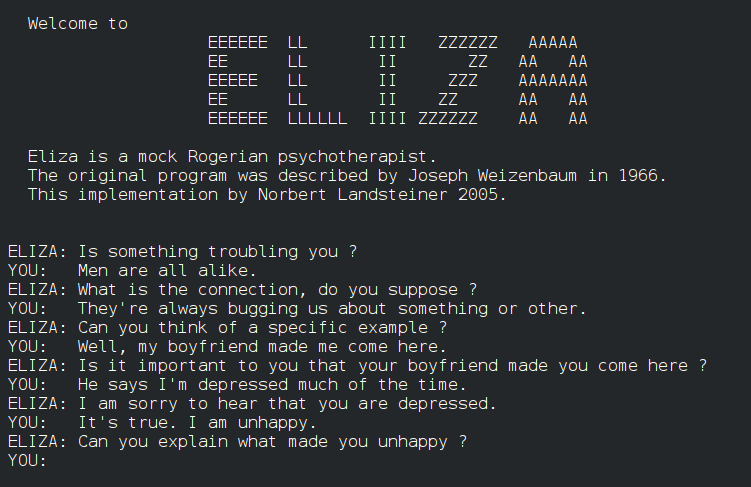
\includegraphics[width=0.75\linewidth]{eliza.png}
        \caption[ELIZA]{ELIZA, an early program for natural language interaction between humans and computers~\cite{wangELIZAChatGPTBrief2024}.}
        \label{fig:eliza}
    \end{wide}
\end{figure}

Even though Weizenbaum already used the term "artificial intelligence" to describe ELIZA~\cite{weizenbaumELIZAComputerProgram1966}, her nature is very different from the modern \glspl{LLM} we know today. He explains ELIZA as follows: "Input sentences are analyzed on the basis of decomposition rules which are triggered by key words appearing in the input text. Responses are generated by reassembly rules associated with selected decomposition rules."~\cite{weizenbaumELIZAComputerProgram1966}. Furthermore, "Keywords and their associated transformation rules constitute the SCRIPT for a particular class of conversation."~\cite{weizenbaumELIZAComputerProgram1966}. These scripts defined both the language (e.g. German or English) and the topic of the conversation via the role ELIZA takes~\cite{weizenbaumELIZAComputerProgram1966}. Weizenbaum found the only "serious" script to be one where ELIZA acts as a psychotherapist~\cite{weizenbaumELIZAComputerProgram1966}, which is the one depicted in \cref{fig:eliza}.

ELIZA works deterministically, as opposed to the probabilistic nature of today's \glspl{LLM}. However, ELIZA shares some abilities with modern \glspl{LLM}: A "rank" was assigned to keywords, so relevant words could be distinguished from less relevant ones~\cite{weizenbaumELIZAComputerProgram1966}. Furthermore, ELIZA was able to understand minimal, specific context via a corresponding script~\cite{weizenbaumELIZAComputerProgram1966}. This is likely why in hindsight, ELIZA is often considered the world's first chatbot~\cite{berryLimitsComputationJoseph2023,shragerELIZAReinterpretedWorlds2024,wangELIZAChatGPTBrief2024}.

Early work in \gls{AI} was mostly theoretical, as both computing power and training data were very limited~\cite{shragerELIZAReinterpretedWorlds2024}. When the internet became prevalent around the year 2000, researchers started compiling internet-scale training datasets~\cite{bankoScalingVeryVery2001,resnikWebParallelCorpus2003,kilgarriffIntroductionSpecialIssue2003}. For the first time, a rich variety of content was available in any language, easily accessible from anywhere in the world. This accelerated the progress in \gls{AI}, and more specifically in \gls{NLP}: In 2011, Apple launched Siri, the first natural language assistant to attract lasting public attentionn~\cite{wangELIZAChatGPTBrief2024}.

In 2017, the introduction of the Transformer architecture for \glspl{LLM} laid the foundation for the popular chatbots we know today~\cite{vaswaniAttentionAllYou2023}. In turn based on the attention mechanism introduced in 2014~\cite{bahdanauNeuralMachineTranslation2016}, it enabled \glspl{LLM} to consider the context a word is in, instead of processing each word in isolation~\cite{vaswaniAttentionAllYou2023,bahdanauNeuralMachineTranslation2016}. Furthermore, each word is weighted with an attention score, allowing the \gls{LLM} to focus on relevant words~\cite{vaswaniAttentionAllYou2023,bahdanauNeuralMachineTranslation2016} - just like ELIZA, but in a vastly different order of magnitude.

In 2019, after initially deeming too dangerous to make public, OpenAI released GPT-2~\cite{hernNewAIFake2019}. With the release of ChatGPT in December 2022, chatbots finally gained widespread popularity in personal, educational and professional use~\cite{wuUnveilingSecurityPrivacy2024}. \gls{AI} assists researchers and engineers~\cite{schmidgallAgentLaboratoryUsing2025} in anything from solving physics equations~\cite{panQuantumManybodyPhysics2025,songLLMFeynmanLeveragingLarge2025} to writing and debugging code~\cite{shiCodeCorrectnessClosing2024,tianDebugBenchEvaluatingDebugging2024,leeUnifiedDebuggingApproach2024,leeGitHubRecentBugs2024}. In education, they can support individualized learning and automate administrative tasks~\cite{mienyeChatGPTEducationReview2025}. In industries like healthcare and e-commerce, chatbots are used in customer service as they provide instant responses and personalized experiences~\cite{wangELIZAChatGPTBrief2024}. As virtually all industries are influenced in one way or another and user acceptance is high~\cite{wangHistoryDevelopmentPrinciples2024,wangELIZAChatGPTBrief2024}, \gls{AI} is here to stay.

\subsection{Making a virtue out of necessity}
\label{sec:makingAVirtueOutOfNecessity}
While there is much more to discuss about the inner workings of \glspl{LLM} and how they relate to other methods in the field \gls{NLP}, this is not the core of this thesis. In this section, we want to focus on problems that come with the common usage of \glspl{LLM} in the form of commercial chatbots. This will show us requirements needed for our implementation of text-based steganography to protect user privacy.

With the vast public attention \gls{AI} has gotten in recent years, its commercialization is in full swing~\cite{soniOpenAIOutlinesNew2025}. As \gls{AI} influences increasingly many aspects of our daily lives, it accesses highly sensitive data. For example, it can be used to analyze social media activity~\cite{sufiSocialMediaAnalytics2023}, evaluate health records~\cite{lovonEvaluatingLLMAbilities2025} or support children in school~\cite{mienyeChatGPTEducationReview2025}. As many \gls{AI} applications need signifcant computing resources, many individuals and organizations are dependent on cloud-based service providers. These service providers may have interest in harvesting our personal data for additional commercial gain~\cite{biddleFacebookEngineersWe2022,mccallumMetaFacebookOwner2023}. Therefore, privacy and security play a central role for long-term viability of \gls{AI}~\cite{guptaChatGPTThreatGPTImpact2023,wuUnveilingSecurityPrivacy2024}.

Commercial chatbots expose many ethical and privacy concerns~\cite{rayBenchmarkingEthicalAlignment2023}. Ethical concerns are centered around pirated training data~\cite{brittainMetaKnewIt2025,vandersarMetaTorrented812025,liesenfeldOpeningChatGPTTracking2023} and working conditions~\cite{perrigoExclusive$2Hour2023}. Privacy issues don't only concern training data, but reach all the way to the end user experience: Malicious users could extract inputs from other users that the \gls{LLM} was trained on, e.g. by jailbreaking via prompt injection or reverse psychology~\cite{guptaChatGPTThreatGPTImpact2023,wuUnveilingSecurityPrivacy2024}. Furthermore, for many users these service providers would not be in their jurisdiction. Foreign law enforcement could therefore demand and obtain access to user data without users being aware of it or having any legal recourse.

We can't solve all of these issues, but we can leverage \glspl{LLM} to combat some of them. We can deduct some requirements for our implementation of text-based steganography from the issues described above:
\begin{itemize}
    \item Our implementation should run the \gls{LLM} locally. This is to ensure data sovereignity by avoiding any chance of leaks from exposing data to a third party.
    \item Our implementation should provide an acceptable performance on today's entry-level smartphones. This is important since running \glspl{LLM} is resource-intensive and we want to target a very diverse user spectrum.
    \item Our implementation should work offline. This means, once the \gls{LLM} is downloaded, no internet connection should be required. This is within the scope of this thesis, as no server backend for sending messages will be implemented.
    \item Preferably, the \gls{LLM} (and any dependencies) should be open source. This may be achieved by making the \gls{LLM} swappable.
\end{itemize}

Especially the last requirement is more sophisticated than one might think. Many \glspl{LLM} are not open source as per \gls{OSI} definition~\cite{tarkowskiDataGovernanceOpen2025,osiOpenSourceAI,gnuprojectWhatFreeSoftware}. This might be due to training datasets or parameter weights not being avaiable, e.g. in the cases of Llama~\cite{metaMetallamaLlamamodels2025,touvronLLaMAOpenEfficient2023} and DeepSeek~\cite{deepseekDeepseekaiDeepSeekR12025,deepseek-aiDeepSeekR1IncentivizingReasoning2025}, or due to incompatible licenses making them source-available~\cite{liesenfeldOpeningChatGPTTracking2023,whiteModelOpennessFramework2024}.

Training datasets not being disclosed limits our ability to make an educated choice considerably. As an increasing amount of data on the internet is generated by \gls{AI}, it makes its way into future training datasets. This can have a poisoning effect on output quality~\cite{alemohammadSelfConsumingGenerativeModels2023,shumailovCurseRecursionTraining2024,martinezUnderstandingInterplayGenerative2023,martinezCombiningGenerativeArtificial2023}.

Alternatively, we could train our own \gls{LLM}. This would unlock promising perspectives on improving cover text quality. For example, we could personalize the \gls{LLM} by fine-tuning it with past text messages of our own~\cite{donnerSimulationMeFinetuning2024,donnerStepStepGuide2024,donnerFinetuningLLMYour2024,donnerFinetuningLLMYour2024a,donnerFinetuningLLMYour2024b}. However this is not only complex~\cite{huLoRALowRankAdaptation2021} and computationally expensive, but also not necessarily privacy-respecting. On one hand, we may avoid leaks through service providers. On the other hand, we would have to get consent from all people whose chat messages are in our training dataset. For example, for an average Computer Science student at TU Darmstadt taking part in a group chat for every lecture, this could mean over a thousand people.
